% This file was created with tikzplotlib v0.10.1.
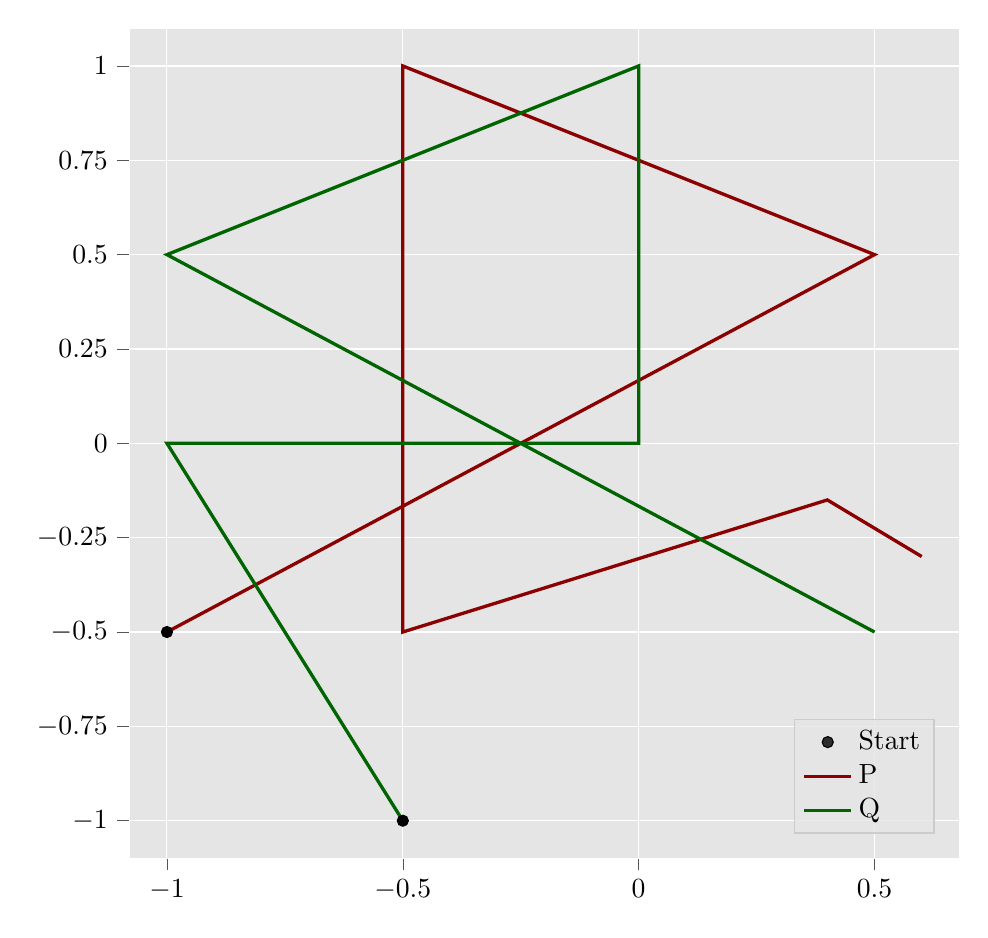
\begin{tikzpicture}

\definecolor{darkgreen}{RGB}{0,100,0}
\definecolor{darkred}{RGB}{139,0,0}
\definecolor{dimgray85}{RGB}{85,85,85}
\definecolor{gainsboro229}{RGB}{229,229,229}
\definecolor{lightgray204}{RGB}{204,204,204}

\begin{axis}[
axis background/.style={fill=gainsboro229},
axis line style={white},
height=\textwidth,
legend cell align={left},
legend style={
  fill opacity=0.8,
  draw opacity=1,
  text opacity=1,
  at={(0.97,0.03)},
  anchor=south east,
  draw=lightgray204,
  fill=gainsboro229
},
minor xtick={},
minor ytick={},
tick align=outside,
tick pos=left,
width=\textwidth,
x grid style={white},
xmajorgrids,
xmin=-1.08, xmax=0.68,
xtick style={color=dimgray85},
xtick={-1.5,-1,-0.5,0,0.5,1},
y grid style={white},
ymajorgrids,
ymin=-1.1, ymax=1.1,
ytick style={color=dimgray85},
ytick={-1.25,-1,-0.75,-0.5,-0.25,0,0.25,0.5,0.75,1,1.25}
]
\addplot [draw=black, fill=black, mark=*, only marks]
table{%
x  y
-1 -0.5
-0.5 -1
};
\addlegendentry{Start}
\addplot [very thick, darkred]
table {%
-1 -0.5
0.5 0.5
-0.5 1
-0.5 -0.5
0.399999976158142 -0.149999976158142
0.600000023841858 -0.299999952316284
};
\addlegendentry{P}
\addplot [very thick, darkgreen]
table {%
-0.5 -1
-1 0
0 0
0 1
-1 0.5
0.5 -0.5
};
\addlegendentry{Q}
\end{axis}

\end{tikzpicture}
